\chapter{Números complejos}
\label{chap:numeros_complejos}

\section{¿Qué es un número complejo?}

EL conjunto de los números complejos represetnado por el símbolo $\mathbb{C}$, es la combinación de números reales e imaginarios. La parte real se puede expresar por un número entero o sus decimales, la parte imaginaria es aquella cuyo cuadrado es negativo.


Los números complejos sirven para dar sentido a la raíz cuadrada de números negativos. Esto permite que ecuaciones de segundo grado con discriminante negativo, puedan ser resueltas. Con esto se abre la puerta a un gran mundo en el que todas las operaciones (excepto dividir entre 0), son posibles.


Las características principales de los números complejos con las siguientes:

\begin{itemize}
    \item Tiene distintas formas de expresarse.
    \item Dos números complejos se consideran iguales cuando tienen mismo componente real e imaginario.
    \item $\mathbb{C}$ conforma un espacio vectorial de dos dimensiones: la de los números reales y la de los imaginarios.
    \item Los números complejos no pueden mantener un orden. Es decir no se puede encontrar una propiedad $>$ o $<$ que un número para todos los números complejos.
\end{itemize}


\section{Representación binómica}

Un número complejo puede expresarse de forma puramente algebraica mediante su \textbf{representación binómica}. Esta forma divide el número en la suma de dos componentes:

\[
    z = a + bi, \quad a, b \in \mathbb{R}, \quad i = \sqrt{-1}
\]

Con esta representación matemática, $a$ constituye la \textbf{parte real} y $b$ la \textbf{parte imaginaria} del número complejo. Si un número carece de parte real ($a=0$), se le denomina imaginario puro.

A partir de la representación binómica de un número complejo se pueden definir a su vez otros dos números complejos fuertemente relacionados:

\begin{itemize}
    \item \textbf{Conjugado:} Se define cambiando el signo de la parte imaginaria, denotándose como $\overline{z} = a - ib$.
    \item \textbf{Inverso:} Se define como $z^{-1} = \frac{a}{a^2 + b^2} - \frac{b}{a^2 + b^2}i$.
\end{itemize}

Al estar expresados en forma binómica, las operaciones aritméticas básicas entre dos números complejos $z_1 = a + bi$ y $z_2 = c + di$ se realizan aplicando las propiedades algebraicas de los números reales y teniendo en cuenta que $i^2 = -1$:

\begin{itemize}
    \item \textbf{Suma y resta:} Se operan las partes reales e imaginarias por separado. Es decir, $z_1 \pm z_2 = (a \pm c) + (b \pm d)i$.
    \item \textbf{Multiplicación:} Se aplica la propiedad distributiva convencional y se simplifica, obteniendo $z_1 \cdot z_2 = (ac - bd) + (ad + bc)i$.
    \item \textbf{División:} Para realizar $\frac{z_1}{z_2}$, se multiplica tanto el numerador como el denominador por el conjugado del denominador ($\overline{z_2}$). Esto elimina la parte imaginaria del divisor, permitiendo separar el resultado final en parte real e imaginaria.
\end{itemize}

\section{Representación geométrica en $\mathbb{R}^2$}

Debido a que la forma binómica de un número complejo $z = a + bi$ está unívocamente definida por dos valores reales ($a$ y $b$), existe una correspondencia natural con el espacio bidimensional $\mathbb{R}^2$. Por ello, para representar gráficamente un número complejo, se utiliza un sistema de coordenadas cartesiano denominado \textbf{plano complejo} (o plano de Argand).

Este plano está formado por dos ejes perpendiculares: un \textbf{eje real} (horizontal) donde se ubica la parte real $a$, y un \textbf{eje imaginario} (vertical) donde se posiciona la parte imaginaria $b$. De este modo, el número complejo puede representarse como el punto $(a,b)$ en dicho plano. A este punto geométrico se le conoce formalmente como el \textbf{afijo} del número complejo.

La figura \ref{fig:PlanoComplejo} muestra cómo este punto se posiciona en el plano en base a sus componentes.

\begin{figure}
    \centering
    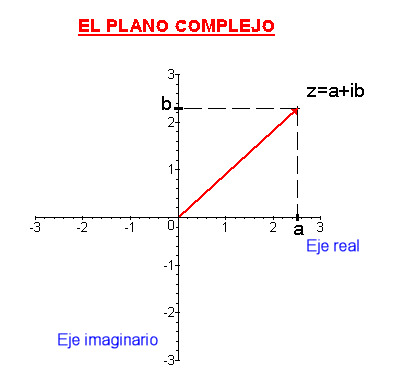
\includegraphics[width=0.5\linewidth]{imagenes/PlanoComplejoRepreGeometrica.jpg}
    \caption{Plano sobre como representar número complejo}
    \label{fig:PlanoComplejo}
\end{figure}

Basándonos en la definición del apartado anterior sobre el inverso y conjugado de un número complejo, al representarlo de forma gráfica queda de la siguiente manera:

\begin{figure}
    \centering
    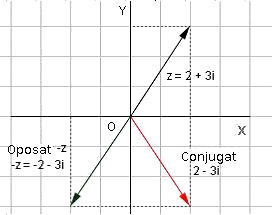
\includegraphics[width=0.5\linewidth]{imagenes/ConjInvCompPlano.jpg}
    \caption{Representación en plano sobre conjugado e inverso}
    \label{fig:ConjInversoPlanoComp}
\end{figure}

\section{Representación forma polar}

Esta representación sirve para destacar los atributos gráficos que tienen los números complejos.\\

\begin{figure}[h]
    \centering
    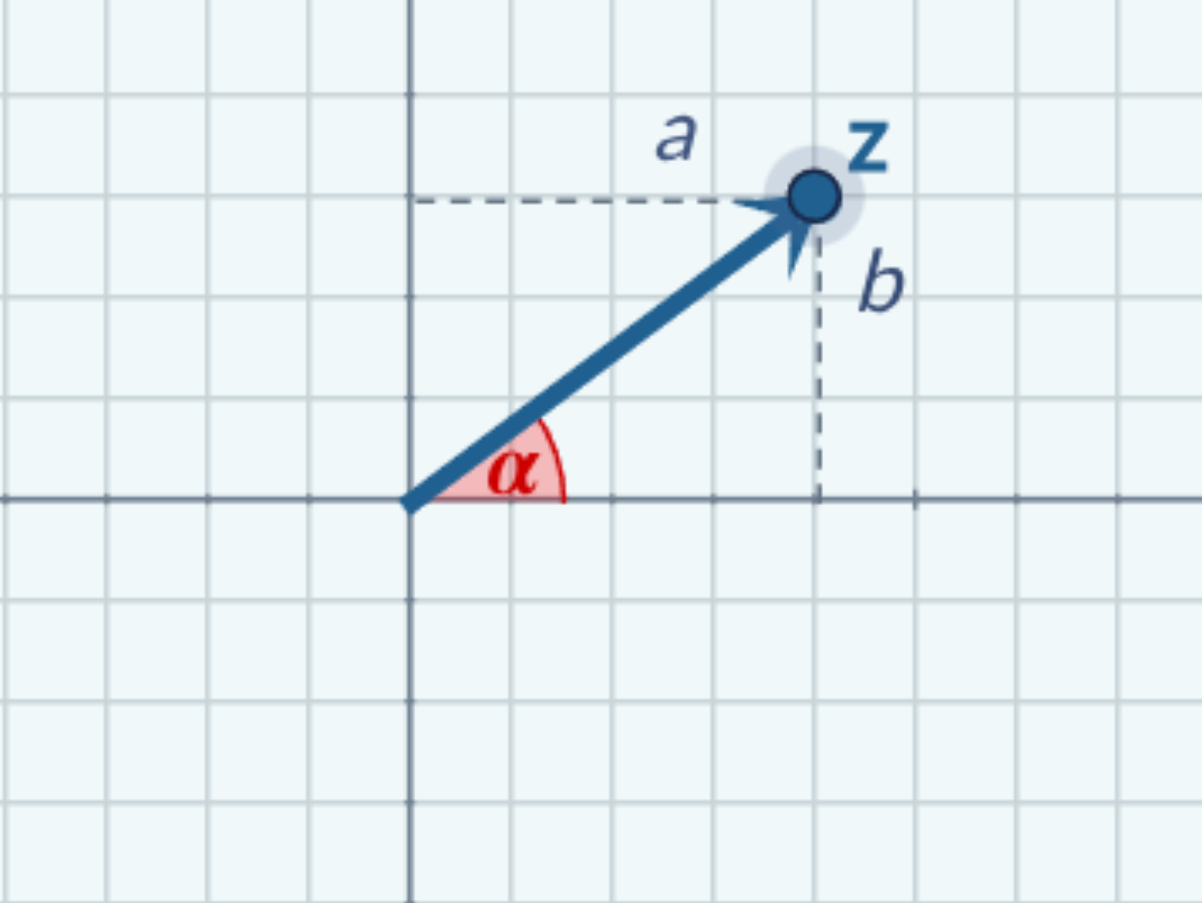
\includegraphics[height=5cm]{imagenes/FormaPolarNumComp.png}
    \caption{Gráfica de la forma polar de un número complejo}
    \label{fig:formaPolar}
\end{figure}

\begin{itemize}
    \item \textbf{Módulo (r):} Distancia del afijo al origen de coordenadas.
    \item \textbf{Argumento (arg(z)):} Ángulo que forma el segmento $\overline{OZ}$ con el semieje positivo medido en el sentido contrario de las agujas del reloj entre 0° y 360°.
\end{itemize}

Con el módulo y el argumento se puede expresar el número complejo \textbf{z} en \textbf{forma polar} de la siguiente forma:
\[
    r_{\alpha} \quad \text{con } r = |z| \text{ y } \alpha = \arg(z)
\]

En base a la forma polar, se puede expresar \textbf{z} en \textbf{forma trigonométrica} de la siguiente manera:

\[
    z = r (\cos \alpha + i \, \sen \alpha), \quad
\]

Esto nos puede servir para pasar de forma polar a forma binómica.\\

\subsection{Operaciones}

Con esta representación, se permite realizar la multiplicación y división de una manera sencilla. Para ello hay que \textbf{expresar los números complejos en forma trigonométrica}.

\begin{itemize}
    \item \textbf{Producto:} $r \cdot r' \, (\cos(\alpha + \beta) + i \, \sen(\alpha + \beta))$\\
          Se observa que el módulo del número complejo es el resultante del producto de los módulos y que el argumento es la suma de los argumentos.

    \item \textbf{Cociente:} $\frac{r}{r'} \, (\cos(\alpha - \beta) + i \, \sen(\alpha - \beta))$
          El resultado del cociente es el cociente de los módulos y la diferencia de los argumentos
\end{itemize}

Por lo que en \textbf{forma polar} quedaría de la siguiente manera:

\begin{itemize}
    \item \textbf{Producto:} $r_\alpha \cdot r_\beta' = (r \cdot r')_{\alpha+\beta}$
    \item \textbf{Cociente:} $\frac{r_\alpha}{r_\beta'} = \left(\frac{r}{r'}\right)_{\alpha - \beta}$
\end{itemize}

Para calcular \textbf{potencia} con exponente natural \textbf{n}, en forma polar, hay que elevar el módulo a \textbf{n} y multiplicar el argumento por \textbf{n}.

\[
    \left( r_\alpha \right)^n = \left( r^n \right)_{n \cdot \alpha}
\]

La \textbf{raíz n-esima} de un número complejo en forma polar, es otro número complejo \textbf{$m_\beta$} que debe de cumplir:

\[
    \left( m_\beta \right)^n = r_\alpha
\]
\[
    m = \sqrt[n]{r} \quad \text{ y } \quad \beta = \frac{\alpha}{n} + \frac{\ang{360} * k}{n}
\]

Todo número complejo tiene n raíces n-ésimas. Todos los afíjos están situados sobre una circunferencia y son los vértices de un polígono regular de n lados. \\

Un ejemplo de forma gráfica calculando la raíz n-esima con lo explicado anterioremnte, es el siguiente:

\newpage
\begin{figure}[h]
    \centering
    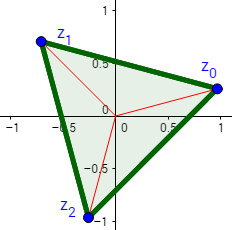
\includegraphics[height=5cm]{imagenes/Raiz3EsimaComplejoPolar.png}
    \caption{Raíz 3-esima del número complejo $z = i + 1$}
    \label{fig:Raiz3esimaComplejo}
\end{figure}

\section{Representación en forma exponencial (Euler)}

El número de Euler ($e$) es un número constante e irracional. Se puede definir a través de la Serie de Taylor.
Este número es la base para resolver ecuaciones relacionadas con el crecimiento exponencial, así como en logaritmos neperianos los cuales sirven para manejar números grandes de una manera simplificada para poder realizar cálculos.\\

La representación del número complejo con el número de Euler, viene dado porque Leonhard Euler aplicó la Serie de Taylor poniéndole la \textbf{$i$} del número imaginario, luego simplificó teniendo en cuenta que \textbf{$i^2 = -1$}. Al aplicar lo comentado, le quedó lo siguiente:

\[
    e^{ix} = \left(1 - \frac{x^2}{2!} + \frac{x^4}{4!} - \dots \right)
    + i \left(x - \frac{x^3}{3!} + \frac{x^5}{5!} - \dots \right)
\] \\

Se dio cuenta que los dos paréntesis de la expresión anterior, es la Serie de Taylor aplicada al \textbf{cos} y \textbf{sen}.

\[
    \cos x = 1 - \frac{x^2}{2!} + \frac{x^4}{4!} - \dots
\]

\[
    \sen x = x - \frac{x^3}{3!} + \frac{x^5}{5!} - \dots
\]\\

Con el seno y coseno, se simplifica en:

\[
    e^{ix} = \cos x + i \, \sen x
\]\\

Este resultado es la representación del número complejo mediante el número de Euler. Además, se le conoce como la \textbf{fórmula de Euler}.